\documentclass[border=15pt, multi, tikz]{standalone}
\usepackage{import}
\subimport{./layers/}{init}
\usetikzlibrary{positioning}
\usetikzlibrary{3d} %for including external image 

\def\ConvColor{rgb:yellow,5;red,2.5;white,5}
\def\ConvReluColor{rgb:yellow,5;red,5;white,5}
\def\PoolColor{rgb:red,1;black,0.3}
\def\DcnvColor{rgb:blue,5;green,2.5;white,5}
\def\SoftmaxColor{rgb:magenta,5;black,7}
\def\SumColor{rgb:blue,5;green,15}
\def\BallColor{rgb:blue,5;green,2.5;white,5}
\def\verdognolo{rgb:green,5;white,2}

\begin{document}
\begin{tikzpicture}
\tikzstyle{connection}=[ultra thick,every node/.style={sloped,allow upside down},draw=\edgecolor,opacity=0.7]
%%%%%%%%%%%%%%%%%%%%%%%%%%%%%%%%%%%%%%%%%%%%%%%%%%%%%%%%%%%%%%%%%%%%%%%%%%%%%%%%%%%%%%%%
%% Draw Layer Blocks
%%%%%%%%%%%%%%%%%%%%%%%%%%%%%%%%%%%%%%%%%%%%%%%%%%%%%%%%%%%%%%%%%%%%%%%%%%%%%%%%%%%%%%%%
\node[canvas is xy plane at x=0] (temp) at (-2.7,0,0) {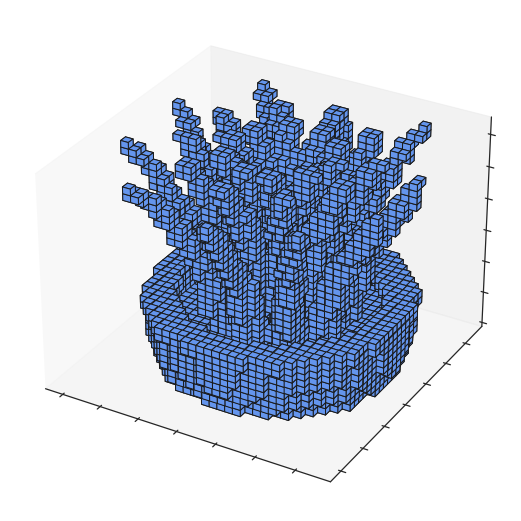
\includegraphics[width=4.5cm,height=4.5cm]{voxel_net.png}};


% conv1_1,conv1_2,%pool1
\pic[shift={(0,0,0)}] at (0,0,0) {RightBandedBox={name=cr1,caption=Conv3D,%
        xlabel={{"1@32x32x32",}},zlabel=,fill=\ConvColor,
        bandfill=\ConvReluColor,%
        height=8,width={8},depth=8}};

% CONV2 +relu + dropout (32,14,14,14)
\pic[shift={(1,1,0)}] at (cr1-east) {RightBandedBox={name=cr2b,%
        xlabel={{" "," "," "," "," "," "," "," "}},
        fill=\ConvColor,bandfill=\ConvReluColor,
        height=3.5,width={3.5,3.5,3.5,3.5,3.5,3.5,3.5,3.5},depth=3.5}};
        
\pic[shift={(1,0,0)}] at (cr1-east) {RightBandedBox={name=cr2,%
        xlabel={{" "," "," "," "," "," "," "," "}},
        fill=\ConvColor,bandfill=\ConvReluColor,
        height=3.5,width={3.5,3.5,3.5,3.5,3.5,3.5,3.5,3.5},depth=3.5}};

\pic[shift={(1,-1,0)}] at (cr1-east) {RightBandedBox={name=cr2c,%
        xlabel={{" "," "," "," "," "," "," "," "}},
        fill=\ConvColor,bandfill=\ConvReluColor,
        height=3.5,width={3.5,3.5,3.5,3.5,3.5,3.5,3.5,3.5},depth=3.5}};
        

 \pic[shift={(1,-2,0)}] at (cr1-east) {RightBandedBox={name=cr2d,caption=Conv3D,%
        xlabel={{" "," "," "," 32@12x12x12"," "," "," "," "}},
        zlabel= stride1,fill=\ConvColor,bandfill=\ConvReluColor,%
       height=3.5,width={3.5,3.5,3.5,3.5,3.5,3.5,3.5,3.5},depth=3.5}};
       
 


% pool + conv
\pic[shift={(1,0,0)}] at (cr2-east) {RightBandedBox={name=cr3,%
        xlabel={{" "," "," "," "," "," "," "," "}},
        fill=\PoolColor,bandfill=\PoolColor,
        height=1.5,width={1.5,1.5,1.5,1.5,1.5,1.5,1.5,1.5},depth=1.5}};

\pic[shift={(1,0.5,0)}] at (cr2-east) {RightBandedBox={name=conv3b,%
        xlabel={{" "," "," "," "," "," "," "," "}},
        fill=\PoolColor,bandfill=\PoolColor,
        height=1.5,width={1.5,1.5,1.5,1.5,1.5,1.5,1.5,1.5},depth=1.5}};
\pic[shift={(1,-0.5,0)}] at (cr2-east) {RightBandedBox={name=conv3b,%
        xlabel={{" "," "," "," "," "," "," "," "}},
        fill=\PoolColor,bandfill=\PoolColor,
        height=1.5,width={1.5,1.5,1.5,1.5,1.5,1.5,1.5,1.5},depth=1.5}};
 \pic[shift={(1,-1,0)}] at (cr2-east) {RightBandedBox={name=conv3b,caption={Conv3D \\  MaxPool3D},%
        xlabel={{" "," "," "," 32@6x6x6"," "," "," "," "}},
        zlabel= ,fill=\PoolColor,bandfill=\PoolColor,%
       height=1.5,width={1.5,1.5,1.5,1.5,1.5,1.5,1.5,1.5},depth=1.5}};

 % pool + conv 2
\pic[shift={(1,0,0)}] at (cr3-east) {RightBandedBox={name=cr4,%
        xlabel={{" "," "," "," "," "," "," "," "}},
        fill=\PoolColor,bandfill=\PoolColor,
        height=1,width={1,1,1,1,1,1,1,1},depth=1}};

\pic[shift={(1,0.3,0)}] at (cr3-east) {RightBandedBox={name=conv4b,%
        xlabel={{" "," "," "," "," "," "," "," "}},
        fill=\PoolColor,bandfill=\PoolColor,
        height=1,width={1,1,1,1,1,1,1,1},depth=1}};
\pic[shift={(1,-0.3,0)}] at (cr3-east) {RightBandedBox={name=conv4b,%
        xlabel={{" "," "," "," "," "," "," "," "}},
        fill=\PoolColor,bandfill=\PoolColor,
        height=1,width={1,1,1,1,1,1,1,1},depth=1}};
 \pic[shift={(1,-0.6,0)}] at (cr3-east) {RightBandedBox={name=conv4b,,%
        xlabel={{" "," "," "," "," "," "," "," "}},
        zlabel= ,fill=\PoolColor,bandfill=\PoolColor,%
       height=1,width={1,1,1,1,1,1,1,1},depth=1}};

       
\pic[shift={(1,0.6,0)}] at (cr3-east) {RightBandedBox={name=cr4b,%
        xlabel={{" "," "," "," "," "," "," "," "}},
        fill=\PoolColor,bandfill=\PoolColor,
        height=1,width={1,1,1,1,1,1,1,1},depth=1}};

\pic[shift={(1,0.9,0)}] at (cr3-east) {RightBandedBox={name=conv4b,%
        xlabel={{" "," "," "," "," "," "," "," "}},
        fill=\PoolColor,bandfill=\PoolColor,
        height=1,width={1,1,1,1,1,1,1,1},depth=1}};
\pic[shift={(1,-0.9,0)}] at (cr3-east) {RightBandedBox={name=conv4b,%
        xlabel={{" "," "," "," "," "," "," "," "}},
        fill=\PoolColor,bandfill=\PoolColor,
        height=1,width={1,1,1,1,1,1,1,1},depth=1}};
 \pic[shift={(1,-1.2,0)}] at (cr3-east) {RightBandedBox={name=conv4b,caption={Conv3D \\MaxPool3D},%
        xlabel={{" "," "," "," 64@2x2x2"," "," "," "," "}},
        zlabel= ,fill=\PoolColor,bandfill=\PoolColor,%
       height=1,width={1,1,1,1,1,1,1,1},depth=1}};

%flatten
\pic[shift={(1,0,0)}] at (cr4-east) {Box={name=fl1,caption=flatten,% 
        xlabel ={{"1x512", " "}} , fill=\DcnvColor, opacity=0.5,%
        height=32, width={2},depth=2}};
%dense1
\pic[shift={(1,0,0)}] at (fl1-east) {Box={name=d1,caption=Dense,% 
        xlabel ={{"128", " "}}, fill=\DcnvColor, opacity=0.5,%
        height=8, width={2},depth=2}};

%dense1
\pic[shift={(1,0,0)}] at (d1-east) {Box={name=d2,caption=Dense,% 
        xlabel ={{"1xN", " "}}, fill=\DcnvColor, opacity=0.5,%
        height=3, width={2},depth=2}};


\node[canvas is xy plane at x=0] (output) at (21,0,0) {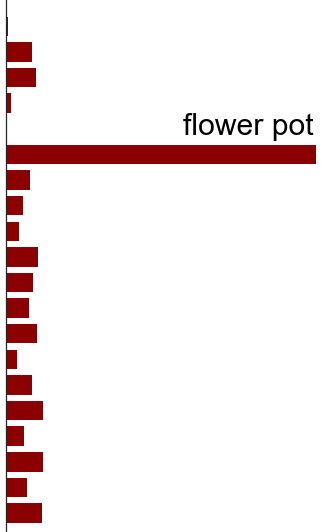
\includegraphics[width = 0.3\textwidth]{distr.png}
};

%%%%%%%%%%%%%%%%%%%%%%%%%%%%%%%%%%%%%%%%%%%%%%%%%%%%%%%%%%%%%%%%%%%%%%%%%%%%%%%%%%%%%%%%
%% Draw connections
%%%%%%%%%%%%%%%%%%%%%%%%%%%%%%%%%%%%%%%%%%%%%%%%%%%%%%%%%%%%%%%%%%%%%%%%%%%%%%%%%%%%%%%%
\draw [connection]  (cr1-east)    -- node {\midarrow} (cr2-west);
\draw [connection]  (cr2-east)    -- node {\midarrow} (cr3-west);
\draw [connection]  (cr3-east)    -- node {\midarrow} (cr4-west);
\draw [connection]  (cr4-east)    -- node {\midarrow} (fl1-west);
\draw [connection]  (fl1-east)    -- node {\midarrow} (d1-west);
\draw [connection]  (d1-east)    -- node {\midarrow} (d2-west);


\end{tikzpicture}
\end{document}\grid